%!TEX root = ../thesis.tex
%*******************************************************************************
%*********************************** Second Chapter *****************************
%*******************************************************************************
\chapter{Introduction to wind turbine modeling and design}
%*******************************************************************************
\hfill
\localtableofcontents
\newpage



%https://eolienne.f4jr.org/eolienne_etude_theorique

%https://www.geotechnique-journal.org/articles/geotech/pdf/2018/04/geotech190004s.pdf

%https://en.wikipedia.org/wiki/Wind-turbine_aerodynamics

%@book{hansen2015aerodynamics,
%  title={Aerodynamics of wind turbines},
%  author={Hansen, Martin OL},
%  year={2015},
%  publisher={Routledge}
%}

%============================================================%
%============================================================%
\section{Introduction}
%============================================================%
%============================================================%

Wind energy is a highly competitive industry with increasing regulations regarding its impact on ecosystems, land-use conflicts, landscapes, or air traffic management \citep{eolien_en_mer_2022}. 
During the long process to win calls for tenders, obtain construction permits, or throughout the wind farm exploitation, an advanced technical understanding of such systems might offer a competitive advantage. 

The operation of offshore wind turbines are driven by multiple physics coupled. 
This behavior results from different external solicitations which are highly turbulent and uncertain. 
Among them, the \textit{metocean} (abbreviation of meteorology and oceanography) environmental conditions play an important role. 
Note that many other types of solicitations also affect the exploitation of offshore wind turbines (e.g., corrosion of the structure, global scour, marine growth, stress concentration factor induced by the manufacturing quality, etc.). 

In this context, numerical models have been developed to certify the structural integrity of OWTs with respect to their solicitations. 
A wind farm project planned at given location should pass different validation procedures established by international standards such as the International Electrotechnical Commission \citep{iec_2019}. 
As wind turbine structures face a large amount of stress cycles in their lifetime (up to $10^8$ for 25 years of operation), this chapter will particularly focus on fatigue damage assessment.


This chapter briefly introduces wind turbine modeling and design, in the following layout: 
Section \ref{sec:metocean_simulation} presents the methods used for wind and wave generation and wake simulation at a farm scale; 
Section \ref{sec:owt_modeling} recalls elements of theory associated with wind turbine modeling; 
Section \ref{sec:owt_design} introduces recommended practices regarding design and operation;
finally, Section \ref{sec:owt_uncertainties} gives a description of the various sources of uncertainties considered in this thesis. 
Considering the standard uncertainty quantification diagram presented in \fig{fig:UQ_methodo}, the material of this chapter is related to the step A (problem specification) and the step B (uncertainty quantification). 
%To go further this general introduction, the reader might refer to the following sources on the different topics 



%============================================================%
%============================================================%
\section{Metocean conditions simulation} \label{sec:metocean_simulation}
%============================================================%
%============================================================%

In the atmosphere, the wind is the air movements caused by the heterogeneous solar heating of Earth's surface. 
Winds usually move from high-pressure to low-pressure regions. 
Earth's rotation also impacts large-scale climate patterns, including winds, according to the well-known Coriolis effect. 
The wind is a highly variable resource, making its exploitation for energy production uncertain. 
This variability is both expressed in space and time with different behaviors depending on the scales studied. 

Regarding large timescales, yearly seasonal fluctuations of wind conditions are well-defined using probability distributions (typically Weibull distributions). 
Predictions at a shorter timescale are usually unreliable beyond a few days ahead. 
Under a few days, the spectral wind energy distribution per time unit is repesented by its power spectral density (PSD). 
Historically, the spectral study of horizontal wind by \citet{van_1957_wind_psd} for timescales between a few seconds and ten days revealed distinct ranges of behaviors. 
The PSD, such as the one illustrated in \fig{fig:wind_psd}, presents three main separated peaks, explaining how the wind energy is split. 
The two first peaks are named ``synoptic'' and ``diurnal'' peak, which respectively correspond to return periods around four days and one day.
While these two peaks are relatively close together, the third peak is completely separated. 
This peak describes the energy related to the wind turbulence, which evolves in the range below ten minutes. 
Considering this energy distribution, wind behaviors are often referred to as ``short-term'' (for turbulent wind) and ``long-term'' (otherwise). 
In wind turbine simulation, ten minutes simulations became a common practice to fully consider turbulent winds. 

Note that the spectrum presented in the research paper of \citet{van_1957_wind_psd} was build from wind measures near New York, USA. 
The same pattern between the three peaks is rather constant between sites, however, the geography (including the surface roughness, the topology, the proximity to the coast, etc.) may affect this distribution. 
At a larger timescale than one year, assessing trends becomes complicated. 
Wind resource assessment over decades are made more uncertain by the human-caused climate change \cite{nagababu_2023_climate_change}, which disrupts large weather trends and the occurrence of extreme events. 

\begin{figure}
    \centering
    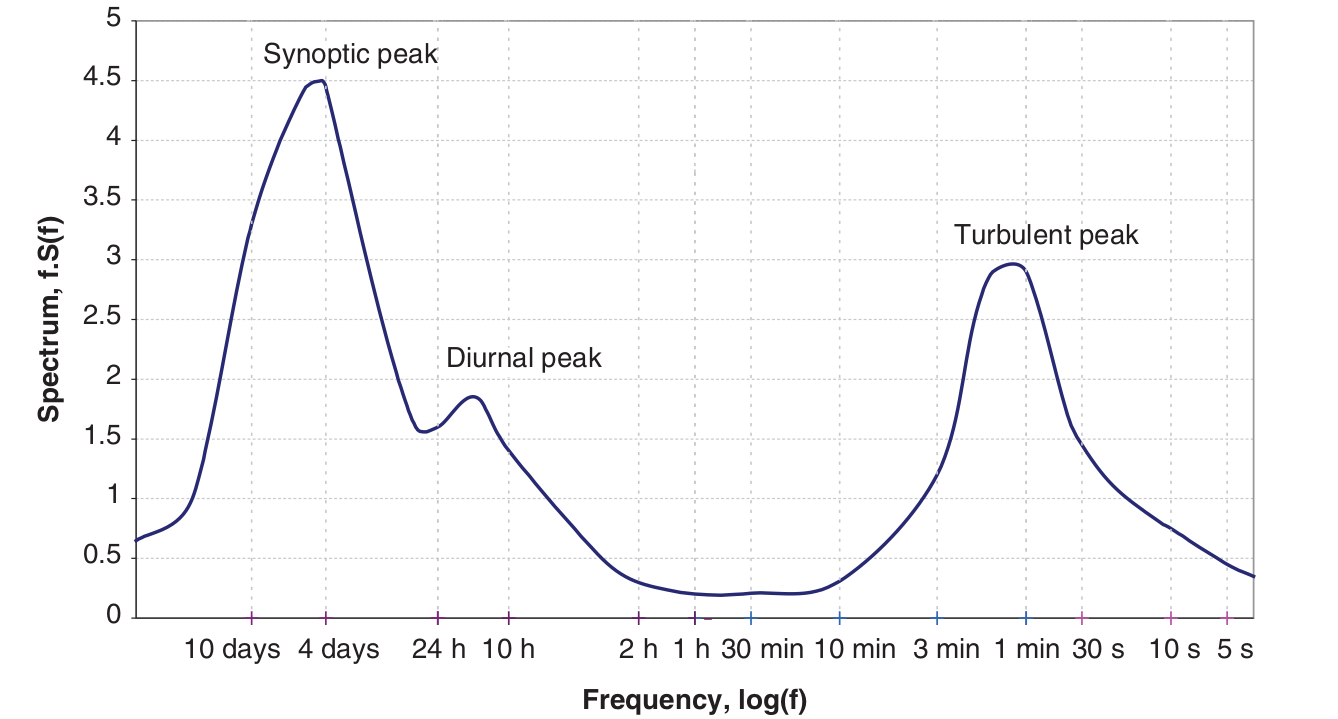
\includegraphics[width=0.7\textwidth]{./part1/figures/wind_spectrum.png}
    \caption{Wind spectrum from Brookhaven, USA (source: \citet{burton_2021_wind_handbook})}
    \label{fig:wind_psd}
\end{figure}


\noindent
\elias{Add something general regrading wave modeling?}



%============================================================%
\subsection{Turbulent wind generation}
%============================================================%

The wind turbulence is a complex and aleatory process, often described as chaotic, since a small perturbation of its initial conditions might have an important impact on the response. 
However, the wind over short-term periods (i.e., ten minutes periods) is usually assumed to be a Gaussian process with constant mean $\overline{U}$ and standard deviation $\sigma_U$ \citep{burton_2021_wind_handbook}. 
Its mean is modeled by the long-term wind conditions (i.e., mean wind speed), often described by a probabilistic model such as a Weibull distribution. 
Note that this assumption is based on the bimodal wind energy distribution observed in \fig{fig:wind_psd}, which might vary at some specific locations. 

The \textit{turbulence intensity} is a commonly used normalized statistic of the wind variability: 
\begin{equation}
    I = \frac{\sigma_U}{\overline{U}}.
\end{equation}

\begin{figure}
    \centering
    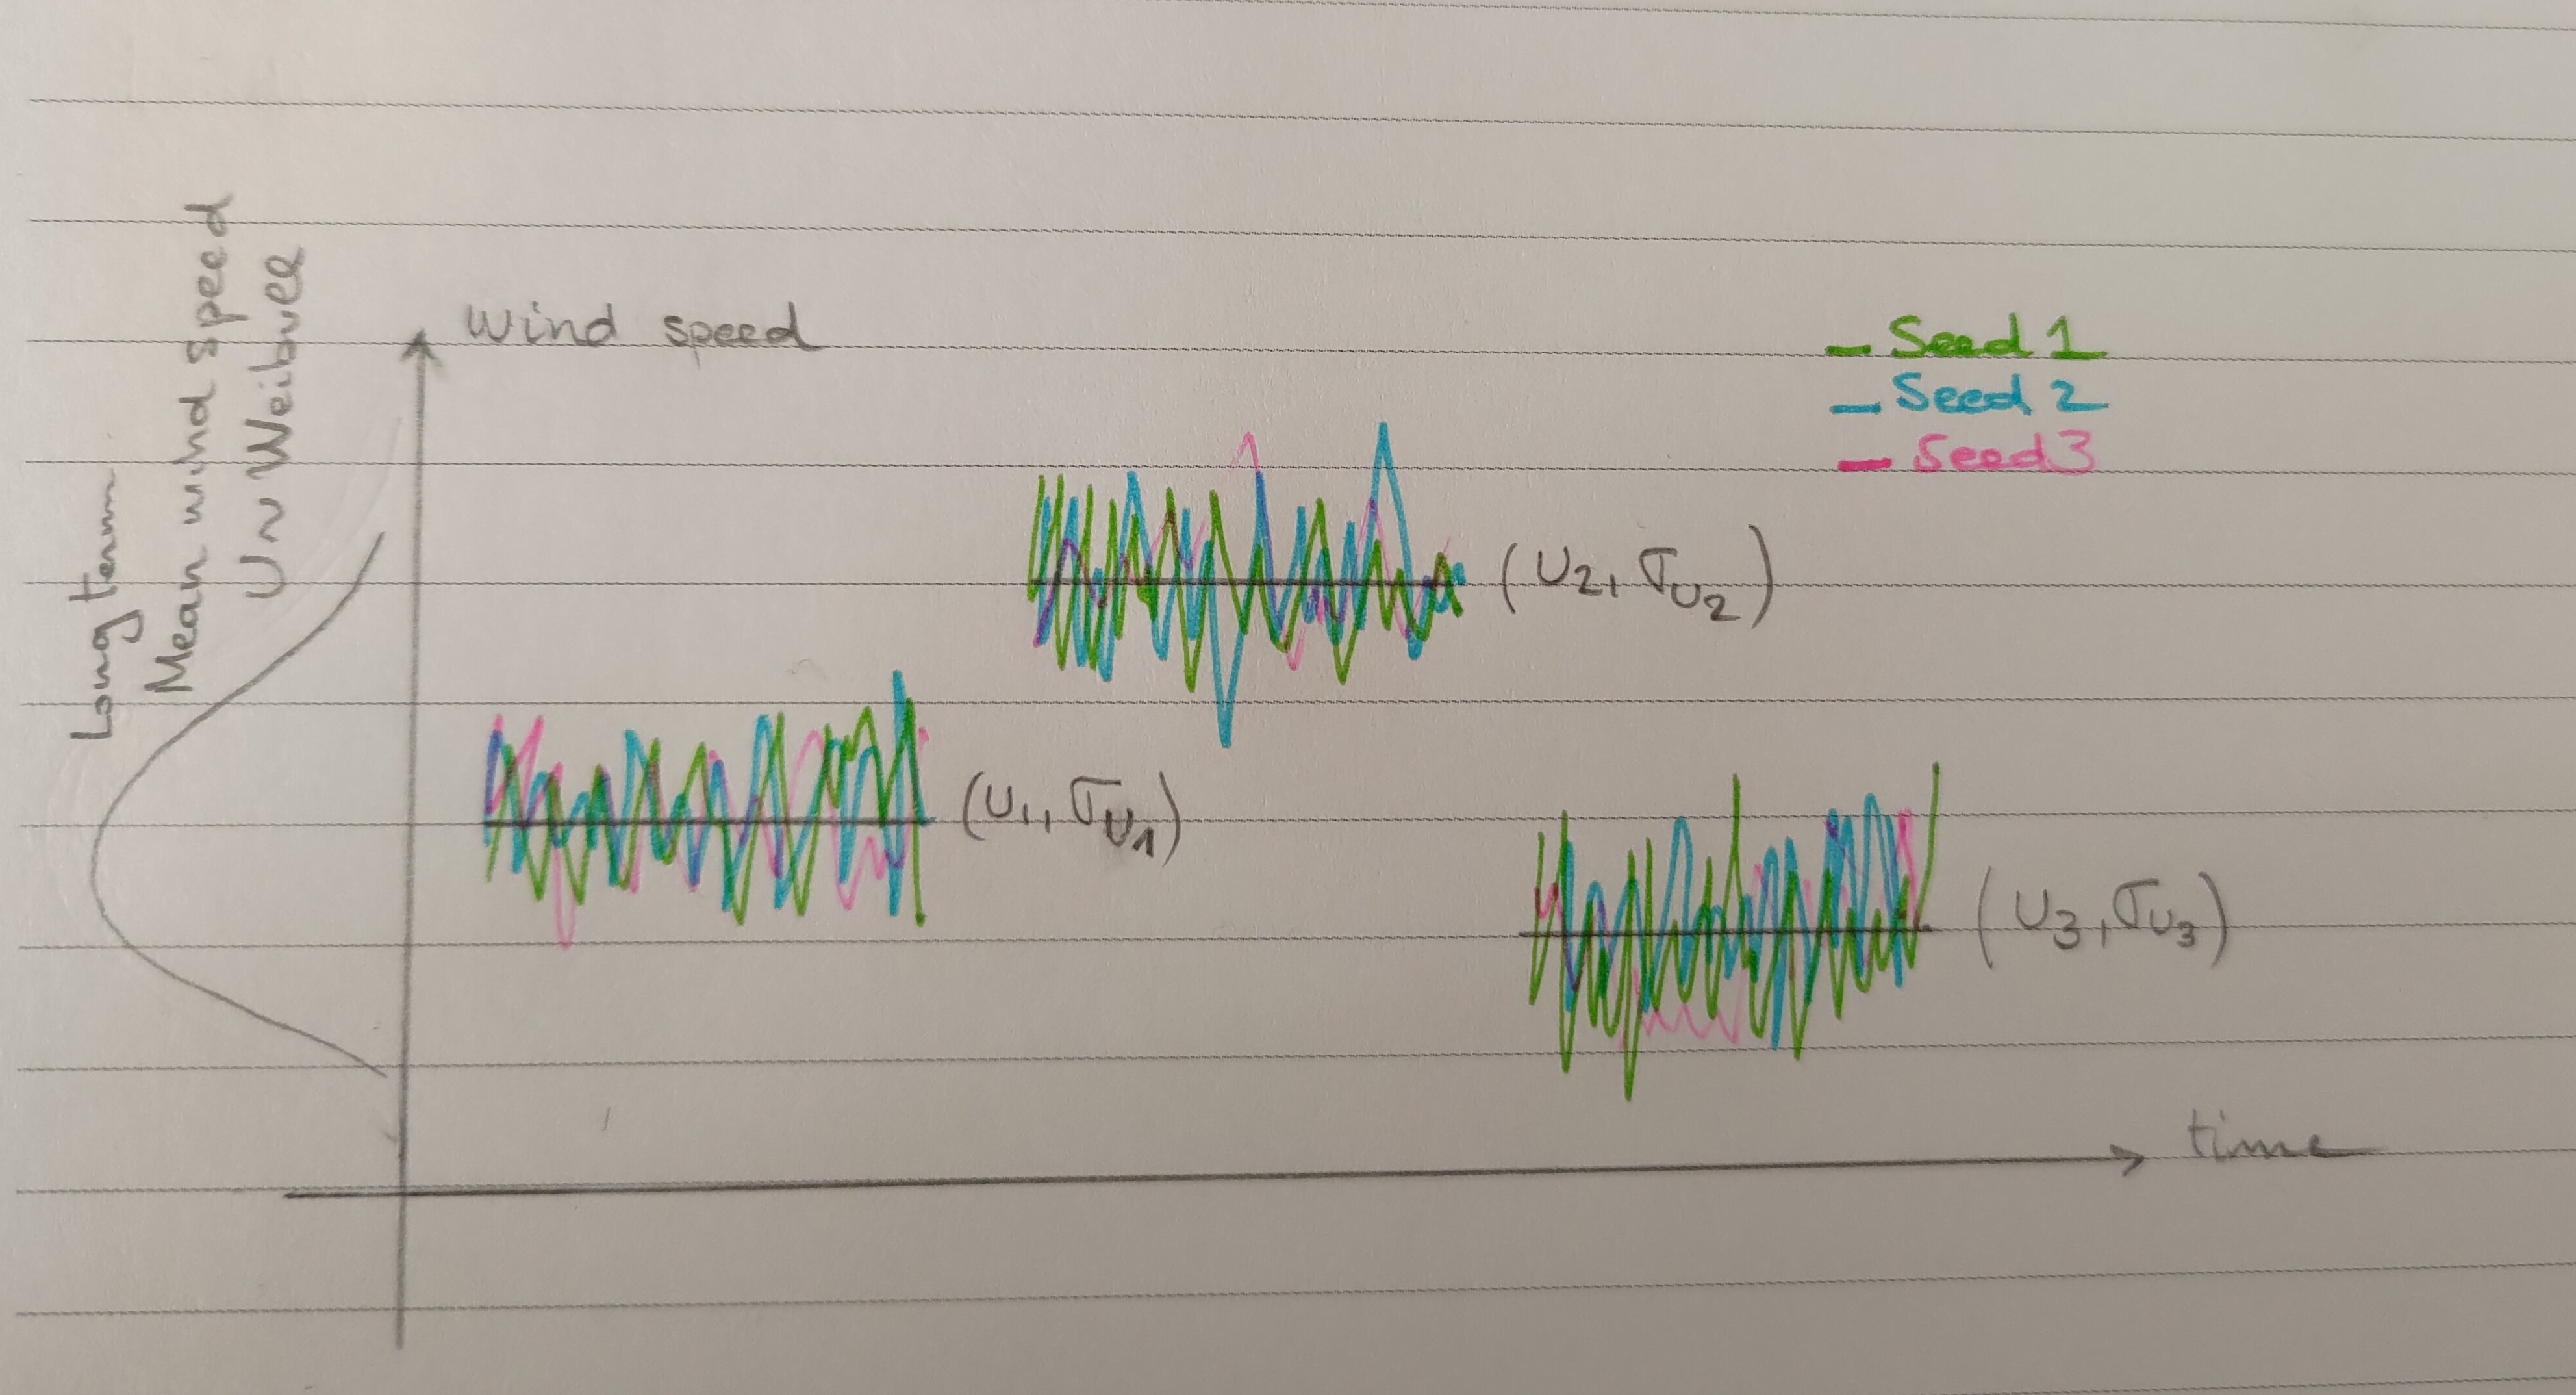
\includegraphics[width=0.7\textwidth]{./part1/figures/wind_long_short_term.jpg}
    \label{fig:wind_long_short_term}
    \caption{\elias{Representation to be confirmed and mentioned in the text}}
\end{figure}

As the wind depends on differences between pressure, humidity, air density, different models exist to represent vertical wind profiles. 
The vertical change in wind conditions is referred to as \textit{vertical wind shear}.
Assuming a constant standard deviation over the altitude, the power law is a widely used approximated shear model \citep{iec_2019}:
\begin{equation}
    \overline{U}(z) = \overline{U}_0 \left(\frac{z}{z_{\mathrm{0}}}\right)^\alpha,
\end{equation}
with $\overline{U}_0$ a well-defined mean wind speed at the height $z_{\mathrm{0}}$ (typically corresponding to a measurement height), 
$z$ the studied height (e.g., the turbine's hub-height), and $\alpha$ the vertical shear coefficient (defined according to measures or standards recommendations). 

To generate a turbulent wind field on a mesh around the turbine, the general mechanism is to apply inverse Fourier transforms on a turbulent wind spectrum.  
Two types of parametric spectrums are commonly used in wind energy: the \textit{Kaimal model} \citep{kaimal_1972} and the \textit{Mann model} \citep{mann_1998}. 
In this thesis, the Kaimal spectrum as defined in \cite{iec_2019} is used for turbulent wind generation over the Cartesian component $k \in \{u, v, w\}$:
\begin{equation}
    S_k(f) = \frac{4 \sigma_k^2 \frac{L_k}{\overline{U}}}{\left(1 + 6 f \frac{L_k}{\overline{U}}\right)^{5/3}},
    \label{eq:kaimal}
\end{equation} 
such that $f$ is the frequency, $\overline{U}$ is the longitudinal mean speed at hub-height, $L_k$ are the Kaimal length scales, and $\sigma_k$ standard deviations (see the complete definition in Annex C of \cite{iec_2019}). 
Along with the Kaimal wind speed spectrum, a spacial coherence model is usually defined in the frequency domain. 
Each couples of nodes in the mesh are correlated, for example, using an exponential coherence model (for further detail in Annex C from \cite{iec_2019}).

In this thesis, the full-field turbulent wind fields (i.e., over a regular mesh) are generated using TurbSim, a software developed by the National Renewable Energy Laboratory (NREL) \citep{turbsim_2009}. 
TurbSim generates time realizations by adapting the spectral method proposed in \citet{veers_1988_sandia} (relying on the inverse Fourier transforms of each component).   
Considering a wind spectrum (e.g., Kaimal model) and a vertical shear model (e.g., power law), TurbSim takes as inputs a mean wind speed, a turbulence standard deviation and a mean wind orientation. 
\fig{fig:turbsim_simu} illustrates the corresponding wind field generated by a ten-minutes TurbSim simulation, considering a set of input long-term conditions. 

\begin{figure}
    \centering
    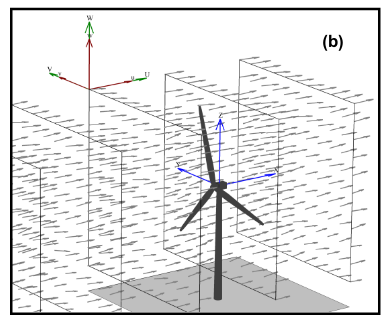
\includegraphics[width=0.5\textwidth]{./part1/figures/turbsim.png}
    \caption{Example of a turbulent wind field generated by TurbSim (source: \citet{turbsim_2009})}
    \label{fig:turbsim_simu}
\end{figure}

In their recent review of the challenges in wind energy, \citep{veers_2019_review} list some limits of the two spectral turbulence models recommended by the standards. 
First, their parameters were fitted using a restricted amount of data \citep{dimitrov_2017_turbulence_models_on_loads}. 
Second, the spacial coherence models associated with Kaimal models showed differences with turbulence measured on site \citep{saranyasoontorn_2004}.  
Finally, recent studies showed that the choice of spectral model impacts the resulting wind turbines loads \citep{doubrawa_2019}. 
These approximations generally tend to overestimate wind flows, leading to conservative designs.

To ensure the most realistic turbulent wind field generation, two research perspectives are actively explored. 
Authors recently developed hybrid methods, including measurement data to enhance spectral models \citep{dimitrov_2017_constrained_turbulence}. 
Alternatively, higher fidelity models were studied in this domain, see for example the use of vortex methods \citep{branlard_2017_book} and large eddy simulations (LES) \citep{doubrawa_2019,bui_2022_mesoscale_LES}.  
Such complex models allow the simulation of mesoscale conditions (e.g., at the farm scale), and extreme transient events (e.g., gusts and storms). 
However, their computational cost is often prohibitive in uncertainty quantification studies. 
When studying the wind resources at a wind farm scale, modeling wind energy losses induced by the turbines' wake becomes essential.


%============================================================%
\subsection{Wake modeling}
%============================================================%

The wake is caused by the extraction of the wind kinetic energy, reducing the wind speed and increasing the turbulence downstream of the turbines (see the illustration in \fig{fig:wake_illustration}). 
In a wind farm, this effect depends on the spacing between turbines, as well as the ambient wind speed and turbulence intensity. 
The turbines positioned at the center of the farm are the most impacted by the wake. 
As a wind farm owner, the consequence of the wake is twofold: a loss of energy production (in the range of 10 to 20 percents depending on the farm), and an increase of fatigue loads (due to the asymmetric loading from the created turbulences).

\begin{figure}
    \centering
    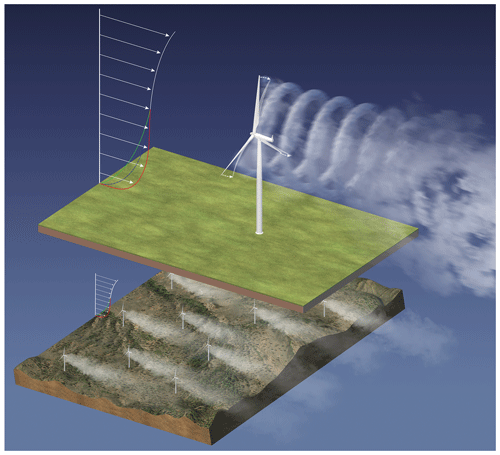
\includegraphics[width=0.5\textwidth]{./part1/figures/wake.png}
    \caption{Illustration of the wake created downstream a wind farm (source: \citet{veers_2019_review})} 
    \label{fig:wake_illustration}
\end{figure}

The initiation of the wake is a complex physical mechanism, however, the wake almost becomes axisymmetric after two turbine diameters downstream. 
At this stage, the wind speed deficit often presents a Gaussian profile centered on the hub \citep{burton_2021_wind_handbook}. 
Numerical models of different fidelities aim at simulating the wake. 
For example, computational fluid dynamics (CFD) models give a detailed description of the wake (including near the turbine) but require high computational efforts. 
In practice, simple analytical models (often called ``engineering models'') are widely used and recommended by standards (see e.g., Annex E in \citet{iec_2019}). 
These models mostly rely the equivalence between the thrust load on the turbine wind energy deficit. 
Since the seminal engineering model proposed by \citet{jensen_1983_wake}, multiple enhancements were proposed. 
A wide benchmark of the wake modeling solutions for different fidelities was performed in \citet{doubrawa_2020_benchmark} and \citet{hiperwind_2023_wp3}. 
The optimal tuning of these engineering models was studied using measurements from a Doppler wind lidar in \citet{zhan_2020_optimal_wake}. 
Different software programs propose wake engineering models, such as: FLORIS (developed by the NREL \citet{fleming_2020_FLORIS}), FarmShadow (developed by IFPEN). 

To take into account the wake effect, control strategies increasingly move from the turbine scale to the farm scale. 
This concept, called ``active wake control'', introduces small yaw misalignments (making the control of turbines individually suboptimal) to optimize the global wake inside the farm \citep{rott_2018_active_control,simley_2020_active_control,meyers_2022_active_control}. 


%============================================================%
\subsection{Irregular wave generation}
%============================================================%

The propagation of wind generated waves has long been studied in hydrodynamics, leading to various wave theories including Airy's, and Stokes'. 
Airy wave theory (also referred to as linear wave theory), models sea states under the hypothesis of small waves relatively to the water depth.  
This spectral approach superposes many regular waves, following the same wave spectrum, to model irregular waves. 
Standard statistics are used in oceanography to represent sea states and their corresponding wave spectra: 
the wave period $T_p$ (with respective frequency $f_p$), and the significant wave height $H_s$ (average over the highest third of the waves measured). 

The most commonly used parametric wave spectrum is called JONSWAP, after the Joint North Sea Wave Project \citep{jonswap_1973}: 
\begin{equation}
    S(f) = \delta \frac{H_s^2}{f} \left(\frac{f_p}{f}\right)^4 \exp\left[-\frac54 \left(\frac{f_p}{f}\right)^4 \right] \gamma^\alpha.
    \label{eq:jonswap}
\end{equation}
The JONSWAP spectrum is a correction of the Pierson-Moskowitz spectrum, adding the peak enhancement factor $\gamma^\alpha$. 
Further details regarding the numerical values to choose in \eq{eq:jonswap} are given in \citet{burton_2021_wind_handbook}. 
An illustration of the two spectra is presented in \fig{fig:jonswap}, revealing the artificial enhancement factor proposed in the JONSWAP model to better fit sea states measurements. 

\elias{Add elements from E.Petrovska p.13 regarding bimodal spectra}

\elias{Add elements in practice: what is done depending on bottom-fixed or floating technology}

\begin{figure}
    \centering
    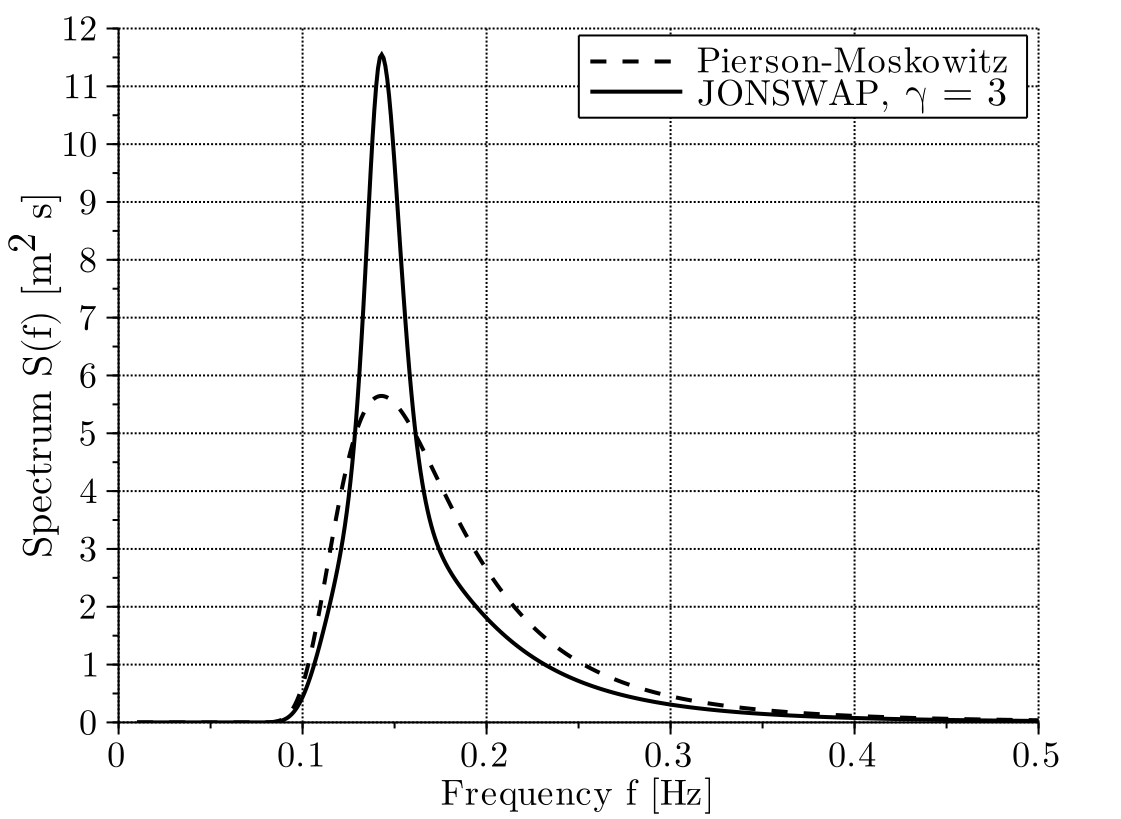
\includegraphics[width=0.5\textwidth]{./part1/figures/jonswap.png}
    \caption{Peirson-Moskowitz and JONSWAP spectra at significant wave height $H_s = 3$
    m and peak period $T_p = 7$ s (source: \citet{milano_thesis_2021})}
    \label{fig:jonswap}
\end{figure}




%============================================================%
%============================================================%
\section{Wind turbine multi-physics modeling} \label{sec:owt_modeling}
%============================================================%
%============================================================%

Offshore wind turbine models are coupling multiple physics such as aerodynamics, hydrodynamics, mechanical elasticity, control and mooring dynamics for floating OWT. 
Similarly to the usual practices from the offshore oil \& gas industry, OWT have been first modeled in the frequency domain. 
At an early design stage, a study in the frequency domain gives a rough idea of the system's feasibility by computing its natural frequencies. 
An OWT should not have its natural frequencies in the same range as the main frequencies of the wave energy spectra. 
Otherwise, such systems can be subject to critical dynamic resonance, leading to their failure.

Beyond this preliminary check, frequency-domain approaches present limits for OWT modeling. 
As they rely on linear assumptions, they are unable to model the non-linearities and transient loading phases \citep{matha_2011_ISOPE}. 
These aspects happen to be essential in the design of OWT \citep{jonkman_2011_ISOPE}. 
As an alternative, the behavior of OWT systems are also simulated in the time domain. 

In the time domain, such systems may be models at different fidelities. 
The diagram in \fig{fig:owt_modeling_fidelities}, illustrates the increasing complexities for two physics involved in OWT modeling (aerodynamics and structural dynamics). 
To perform an uncertainty quantification around a wind turbine model, its fidelity is preferably low. 
At the wind turbine scale, the numerical model studied in this work is actually a chain of three models executed sequentially. 
Note that the wake should also be considered at the wind farm scale, as described earlier. 

\begin{figure}
    \centering
    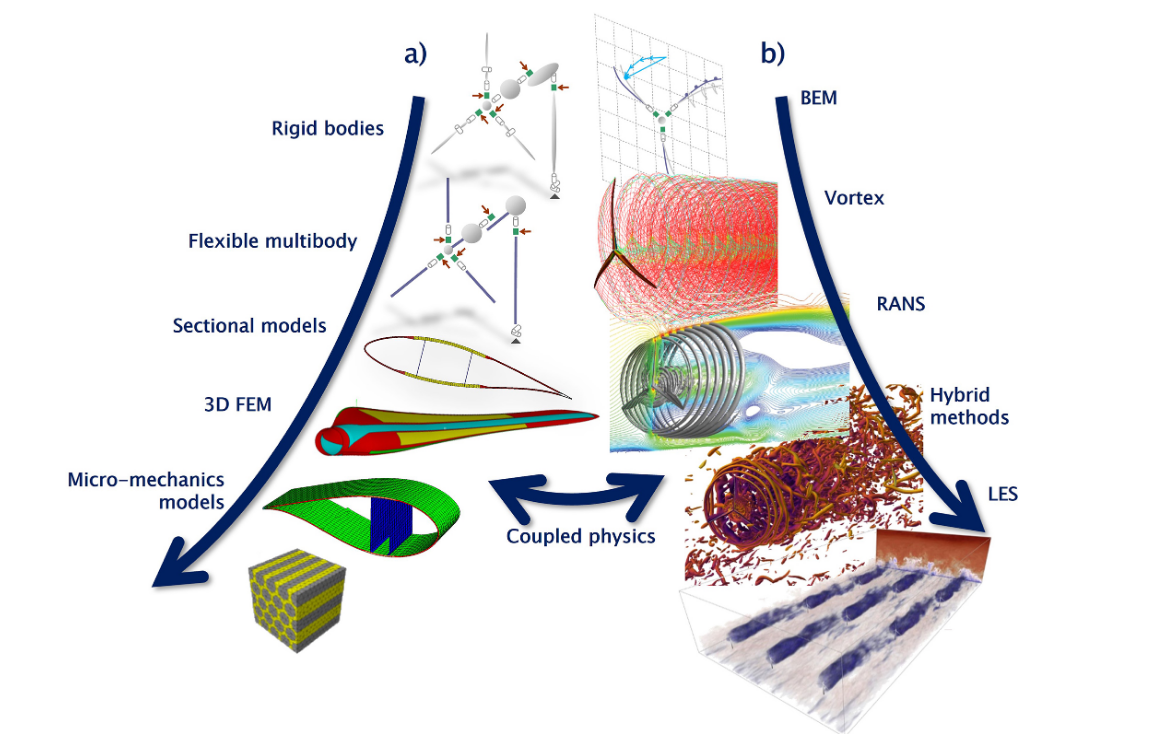
\includegraphics[width=0.7\textwidth]{./part1/figures/OWT_modeling_fidelities.png}
    \caption{Hierarchy of structural (a) and aerodynamic (b) wind energy systems models (source: \citet{veers_2019_review})}
    \label{fig:owt_modeling_fidelities}
\end{figure}

\paragraph{Equation of motion}

\elias{see the equation 1.3 from Milano and the time integration with Newmark scheme}


%============================================================%
\subsection{Aerodynamics of horizontal axis wind turbines}
%============================================================%

The blade element momentum theory mixes different concepts to compute the aerodynamic forces on the rotating blades of the wind turbine.
In this coupled physics models, the aerodynamics affects the structural response and vise-versa. 
To solve this problem, algorithms used in DIEGO first assess displacement of elementary blades, to recover the lift and drag coefficients. 
The elementary loads are then integrated over each blade and communicated to the structure's finite element model (FEM).


\paragraph{Momentum theory.}
%------------------------------------------------------------%
At the core of wind turbine's aerodynamics, the concept of \textit{momentum theory}, also called \textit{actuator disk theory} assumes that the air stream passing thought the rotor disk is bounded by a stream tube of circular surface (not mixing with the ambient air). 
\fig{fig:actuator_disk} is a longitudinal representation of the actuator disk and the way it affects the air stream upstream and downstream the rotor. 
The associated momentum theory assumes the conservation of airflow at any cross-section (of area $A$) during a time period. 
Through the actuator disk, the wind speed slows down and a drop in static pressure is created, at the origin of the wake. 
This pressure drop generates an axial force (called \textit{axial thrust force}) and a torque on the actuator disk.

\begin{figure}[!h]
    \centering
    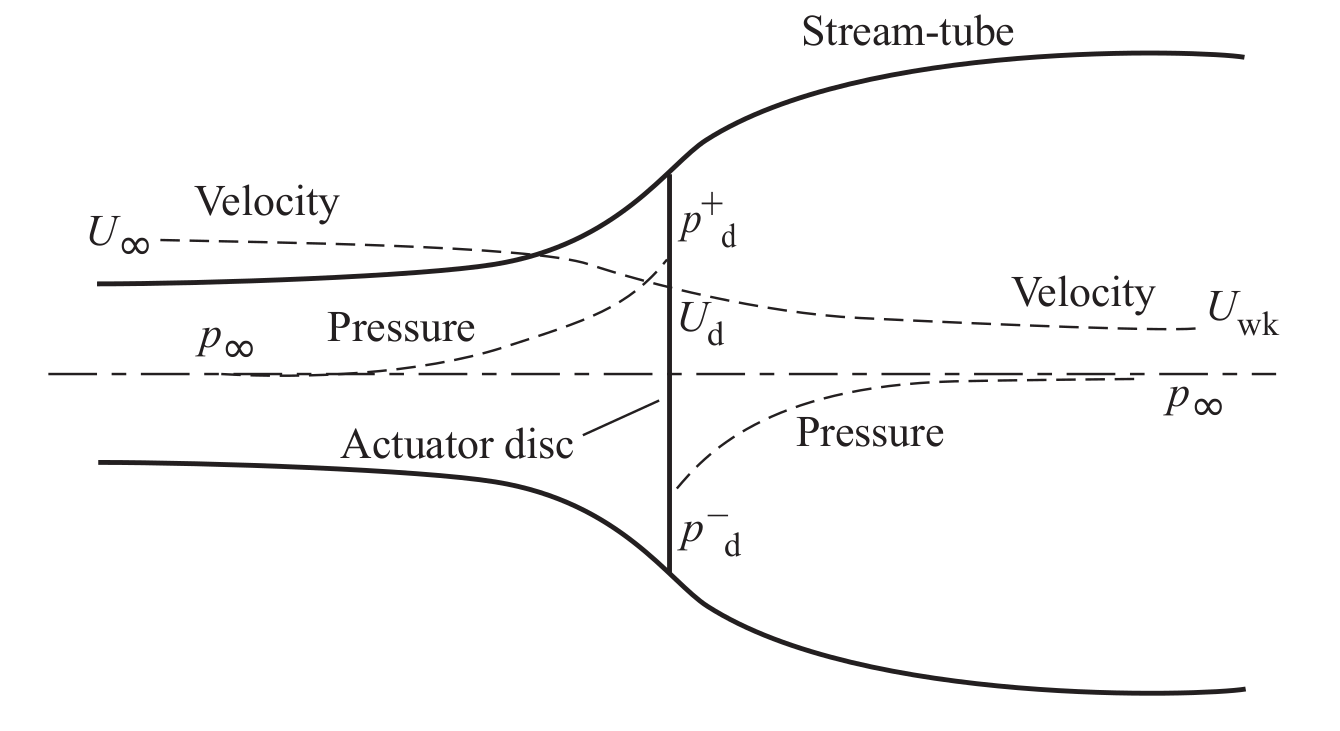
\includegraphics[width=0.6\textwidth]{./part1/figures/actuator_disk.png}
    \caption{Actuator disk model of the energy extraction (source: \citet{burton_2021_wind_handbook}). Longitudinal evolution of the air pressure and wind speed along the wind stream.}
    \label{fig:actuator_disk}
\end{figure}
Considering the upstream flow, the flow at the rotor disk and the airflow in the wake, respectively denoted by the subscripts $\{\infty, d, \mathrm{wake}\}$, the following equality comes:  
\begin{equation}
    \rho A_\infty U_\infty = \rho A_d U_d = \rho A_{\mathrm{wake}} U_{\mathrm{wake}},
\end{equation}
where $U$ is the wind speed, $A$ the stream-tube area, and $\rho$ the air density. 
The wind speed in at the rotor disk can be expressed using the induction factor $a$ in the following expression: 
\begin{equation}
    U_d = U_\infty (1 - a), \, 0\leq a \leq 1.
\end{equation}
Using the momentum theory and Bernoulli's incompressible flow equation, one can express the aerodynamic thrust $T$ and power $P$ (see \citet{milano_thesis_2021}): 
\begin{subequations}
    \begin{align}
        T&=(p_d^+ - p_d^-) A_d = 2 \rho A_d U_\infty^2 a (1- a)\\
        P&= T U_d = 2 \rho A_d U_\infty^3 a (1- a)^2
    \end{align}
    \label{eq:momentum_theory}
\end{subequations}
The widely used power coefficient (respectively thrust coefficient) is the ratio of the power captured by the turbine against to the total kinetic wind power available in the stream tube: 
\begin{subequations}
    \begin{align}
        C_P &= \frac{P}{\frac12 \rho A_d U_\infty^3} = 4a (1-a)^2,\\
        C_T &= \frac{T}{\frac12 \rho A_d U_\infty^2} = 4a (1-a). 
    \end{align}
\end{subequations} 
Betz's law is a theoretical limit value of the power coefficient, obtained by cancelling the power coefficient gradient. 
To this day, no wind turbine has exceeded this limit value: $C_P^{\mathrm{Betz}} = 0.593$ \citep{burton_2021_wind_handbook}.  



\paragraph{Blade element theory.}
%------------------------------------------------------------%
Assuming a purely two-dimensional flow (meaning that the forces are only determined by the lift and drag coefficients), the blade element theory expresses the thrust $\dd T$ and torque $\dd Q$ applied on a blade element.

Let us consider a wind turbine with $B$ blades, with pic length R and pitch angle $\beta$. 
Assuming the blade element represented in \fig{fig:blade_theory} at the blade length $r$, with airfoil chord $c$, angle of attack $\alpha$,  lift $C_L$ and drag $C_D$ coefficients, lift $L$ and drag $D$ forces, and the axial and tangential induction factors $a$ and $a'$. 
Under these assumptions, the axial thrust and torque exerted on a blade element are:
\begin{subequations}
    \begin{align}
        \dd T &= \frac12 \rho W^2 B\, c \left(C_L \cos(\varphi) + C_D \cos(\varphi)\right) \dd r,\\
        \dd Q &= \frac12 \rho W^2 B\, c \left(C_L \sin(\varphi) + C_D \sin(\varphi)\right) \dd r.
    \end{align}
    \label{eq:blade_element}    
\end{subequations}

\begin{figure}[h!]
    \begin{subfigure}[b]{0.5\textwidth}
        \centering
        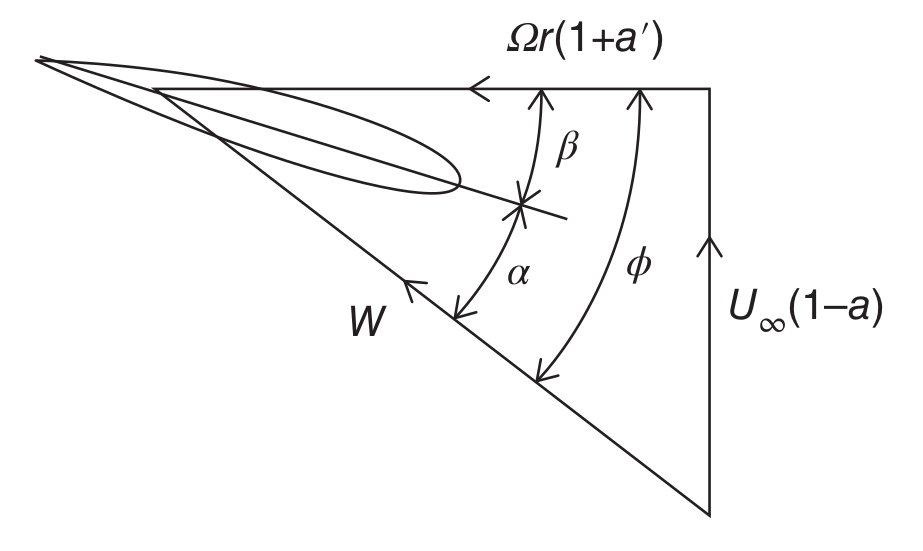
\includegraphics[height=0.15\textheight]{./part1/figures/speed_triangle.png}
        \caption{Speed triangle}
    \end{subfigure}
    \begin{subfigure}[b]{0.5\textwidth}
        \centering
        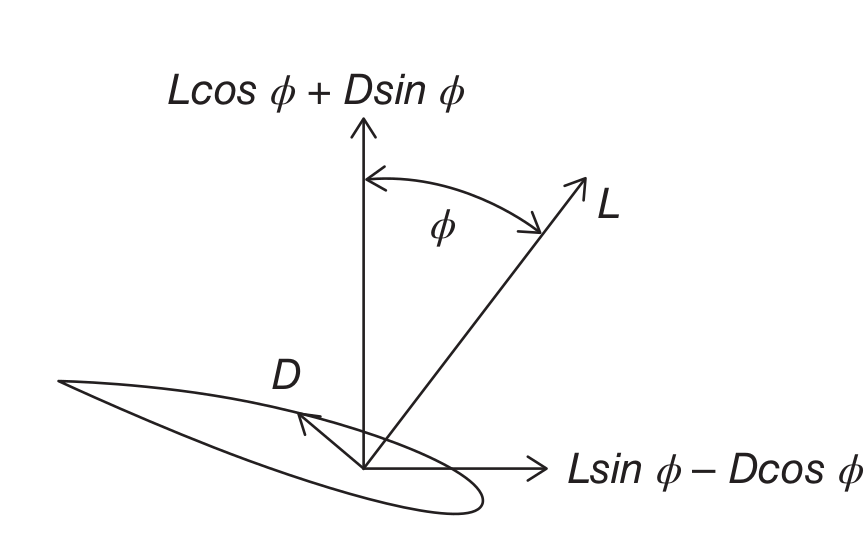
\includegraphics[height=0.15\textheight]{./part1/figures/aerodyn_blade.png}
        \caption{Aerodynamic forces}
    \end{subfigure}
    \caption{Blade element forces. With the lift and drag forces $L$ and $D$, the flow angle $\phi$, the pitch angle $\beta$ and the angle of attack $\alpha$ (source: \citet{burton_2021_wind_handbook}).}
    \label{fig:blade_theory}
\end{figure}
\textit{Blade element momentum theory} (BEMT) combines the results from blade element theory in \eq{eq:blade_element} with the results from momentum theory in \eq{eq:momentum_theory} to obtain the induction factors $a$ and $a'$. 
The resolution of this sytem of equations is often solved by iterative approaches (e.g., \cite{dai_2011_BEMT}). 
Global axial thrust over the blade are then computed by integrating the elementary loads over all the elements. 
Note that various corrections are applied to the BEMT model, for example to take into account the non-homogeneous loss of momentum over the rotor disk. 
The BEMT also fails to model non-linear aerodynamic effects, occurring with sudden change of angle of attack. 
Such effects are sometimes called ``dynamic stall'' and are represented in DIEGO by the Beddoes-Leishman model (see \citet{burton_2021_wind_handbook} for further details).  


%============================================================%
\subsection{Hydrodynamics}
%============================================================%

Morison's equations is a widely-used semi-empirical model to assess the hydrodynamic forces on thin fixed structures such as offshore oil platforms and wind turbines. 
Considering a slender cylindrical structure of diameter $D$, a flow velocity $u(t)$, the drag and inertial coefficients $C_m$ and $C_D$, the axial force (parallel to the flow direction) is given by:   
\begin{equation}
    F\,=\,C_{m}\,\rho \,{\frac {\pi }{4}}D^{2}\,{\frac{\dd u}{\dd t}}\,+\,C_{d}\,{\frac 12}\,\rho \,D\,u\,|u|.
\end{equation}
Standard values for the drag and inertial coefficients are often considered \citep{dnv_2013_offshore_design}. 
DIEGO uses Morison’s equation together with first order potential solution to perform hydrodynamical simulations in the time domain.
An extended introduction to hydrodynamics of fixed slender structures, as well as large floating structures is given in the Chapter 1 from \citep{milano_thesis_2021}.  

%============================================================%
\subsection{Control}
%============================================================%

To maximize their energy production under turbulent wind conditions, wind turbines rely on their control systems. 
This aspect of wind turbines is usually kept confidential by manufacturers, as it gives them a competitive advantage.  
Nevertheless, the general control mode on a wind turbine depends on the wind speed. 
Two main ranges of operation are usually defined: first between the cut-in and rated wind speed, second between the rated and cut-off wind speed. 
Let us then recall the wind turbine power derived from the momentum theory: 
\begin{equation}
    P = \frac12 \rho A_d U_\infty^3 C_p(\lambda, \beta), 
    \label{eq:power_wt}
\end{equation}
with the power coefficient $C_p$, function of the pitch angle $\beta$ and the blade tip speed ratio $\lambda$, defined between the tangential speed on top of the blade and the wind speed: $\lambda = \frac{\Omega \, R}{U_\infty}$, for the rotation speed $\Omega$ and a rotor radius $R$. 

\paragraph{Below the rated wind speed.}
The goal of the control system in this speed range is to extract as much power as available. 
A control strategy among the family of the \textit{maximum power point tracking} can be deployed \citep{abdullah_2012_control_review}.   
For example, the ``power signal feedback'' uses the electromagnetic torque to control the power. 
This method first computes the maxima of the extracted power as a function of the rotation speed (using \eq{eq:power_wt}), for different speed values. 
Then, for a measured wind rotation speed, the system can determine the reference maximal power. 
Considering this reference power, a controller (such a proportional integral controller) intends to match the generated power with the reference by acting on the electromagnetic torque. 


\paragraph{Above the rated wind speed.}
The control system switches to a \textit{power limiting} mode by increasing the blades' pitch angle. 
By operating on the pitch, the rotation speed and the power produced are kept at their nominal values. 
This control is also often realized by a proportional integral system \citep{bossanyi_2003_pitch_control}. 

A more exhaustive description of wind turbines control systems is available in Chapter 8 from \citet{burton_2021_wind_handbook}. 
The more recent strategies often consider the control at the farm scale. 
As explained earlier, the operation of one turbine affects the others via the effect of its wake. 
Moreover, since the wind energy production becomes important in the electric mix, its production might be limited to respect the stability of the grid (e.g., frequency constraints).  
The work of \citet{gionfra_2018_control} studied the optimal control of wind farms considering the effects of the wake and the grid restrictions. 

%============================================================%
\subsection{Structural dynamics}
%============================================================%

The structural elements of modern wind turbines, such as the tower and the blades, compose a dynamic system subject to important elastic deformations. 
Modeling an operating wind turbine therefore requires rigid body dynamics and nonlinear elastic deformations. 
All together, various approaches were developed to model the structural dynamics of wind turbines: modal analysis, multibody methods and finite element methods (FEM). 
At the stage of preliminary designs, modal approaches can be used to model the dynamics under linear assumptions \citep{hegseth_2019_modal_FOWT}. 
The tower's natural frequencies assessed by a modal analysis can be compared with the wind, waves, and the rotor's frequencies. 
As illustrated in \fig{fig:modal_analysis}, the structure's natural frequency (denoted by $f_0$) should not coincide with the main excitation frequencies to avoid critical dynamic resonance.
In the case of a wind turbine, the rotor imbalance creates a first dynamic load of frequency $f_{1P}$, while the blades passing in front of the tower generate a second excitation of frequency $f_{3P}$.  
The \textit{soft-stiff} design strategy places the structure's natural frequency between the two rotor frequencies (i.e., $f_{1P} < f_0 < f_{3P}$ as described in \fig{fig:modal_analysis}). 
%\elias{Note that the wave spectrum is represented with a multimodal distribution}
\begin{figure}
    \centering
    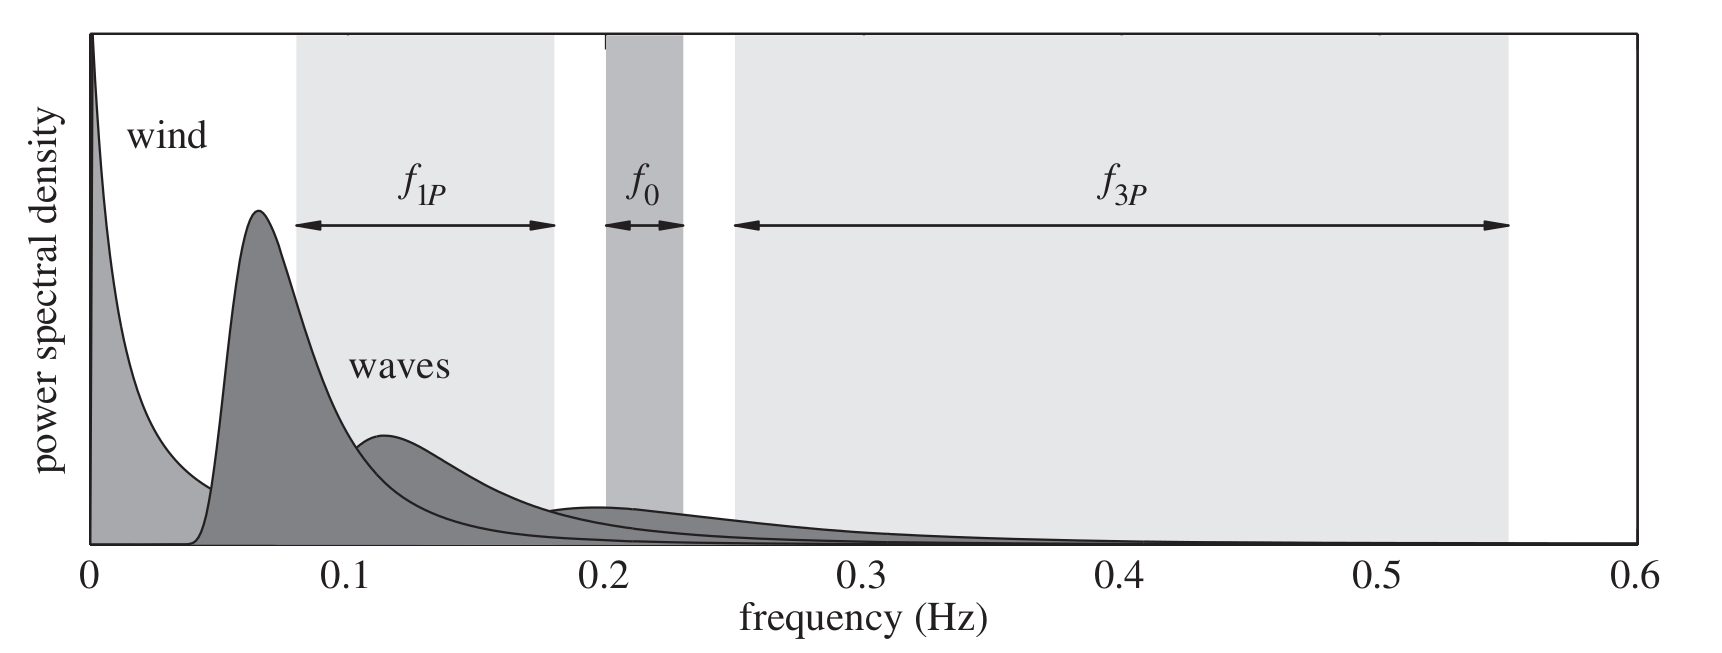
\includegraphics[width=0.75\textwidth]{./part1/figures/modal_analysis.png}
    \caption{Illustration of a soft-stiff design strategy, placing the structure's natural frequency $f_0$ away from the wind and wave power spectra, and the rotor excitation frequencies $f_{1P}$ and $f_{3P}$ (source: \citet{kallehave_2015_modal}).}
    \label{fig:modal_analysis}
\end{figure}

Beyond early design, modal analysis does not model transient loading phases and their corresponding non-linearities. 
For a higher fidelity, simulations in the time domain using flexible multibody approaches are commonly used to describe the nonlinear dynamics \citep{holm_2009_multibody,alsolihat_2018_flexible_multibody}.
DIEGO implements such an approach by combining rigid multibody dynamics with a deflection model based on Lagrangian equations \citep{milano_thesis_2021}. 
\citet{otter_2022_owt_modeling_review} reviews the state-of-the-art of numerical and experimental modelling techniques for multi-physics OWT systems.

%============================================================%
\subsection{Fatigue damage}
%============================================================%
This section discusses the damage assessment defined by the standard \cite{dnv_fatigue_2016}. 
Damage assessment can be divided into four steps: 

\begin{enumerate}
    \item Compute the equivalent Von Mises stress time series;
    \item Identify the stress cycles using rainflow counting;
    \item Define the Stress - Number of cycles curve corresponding to the material;
    \item Compute the damage using Miner's rule.
\end{enumerate}

%The rainflow counting is a tool used to identify the stress cycles from a uniaxial stress time series. 
Since stress is multiaxial in the local coordinate system, the equivalent Von Mises stress is computed, turning a multiaxial stress into an equivalent uniaxial stress. 
This first step is necessary since fatigue laws are mostly established for uniaxial stresses. 
The following expression gives the Von Mises stress for a Cauchy stress tensor:
\begin{equation}
    \sigma _{\mathrm{VM}}={\sqrt{{\frac {1}{2}}\left[(\sigma _{11}-\sigma _{22})^{2}+(\sigma _{22}-\sigma _{33})^{2}+(\sigma _{33}-\sigma _{11})^{2}\right]+3\left(\sigma _{12}^{2}+\sigma _{23}^{2}+\sigma _{31}^{2}\right)}}.
\end{equation}
Note that in the mechanical model, the hypothesis of ``plane strain'' is considered, meaning that the Cauchy stress tensor $\underline{\underline{\sigma}}$ can be written as below:

\begin{equation}
    \underline{\underline{\sigma}} = \begin{pmatrix}
                            \sigma_{11} & \sigma_{12} & 0\\
                            \sigma_{21} & \sigma_{22} & 0\\
                            0 & 0 & \sigma_{33}
                            \end{pmatrix},
\end{equation}
which simplifies the expression of the Von Mises stress:
\begin{equation}
    \sigma _{\mathrm{VM}}=\sqrt{{\frac {1}{2}}\left[(\sigma _{11}-\sigma _{22})^{2}+(\sigma _{22}-\sigma _{33})^{2}+(\sigma _{33}-\sigma _{11})^{2}\right] + 3 \sigma _{12}^{2}}.
\end{equation}

After computing the equivalent Von Mises stress time serie, one can identify the fatigue loading cycles. 
The usual method to identify fatigue stress cycles is rainflow counting \citep{dowling_1972}. 
Fatigue stress cycles are only defined by their amplitude (also called ``range''), regardless of their mean value or their chronology. 
Rainflow counting returns a list of stress ranges identified denoted by $s$ in what follows. 
The ``Stress - Number of cycle'' curve (also called ``W\"ohler curve'') allows one to estimate the number of similar stress cycles necessary to reach a fatigue ruin for a defined stress cycle amplitude. 
A well admitted simplification of the W\"ohler curve is to consider it as log-linear on two parts. 
The W\"ohler curve is generally defined as:
\begin{equation}
    \log(N_{\mathrm{c}}) = \log(a) - m \log(s).
\end{equation}

\noindent One can therefore introduce the following function for each segment of the W\"ohler curve: 
\begin{equation*}
N_{\mathrm{c}} = W(s)= \left\{
    \begin{array}{ll}
        a_{1} s^{-m_1}, & \mbox{for}~ s \in [s_{\mathrm{min}}, s_{\mathrm{e}}] \\
        a_{2} s^{-m_2}, & \mbox{for}~ s \in [s_{\mathrm{e}}, s_{\mathrm{max}}]
    \end{array}
\right.
\end{equation*}

Where $N_{\mathrm{c}}$ is the predicted number of cycles to failure for stress range $s$, $m$ is the negative inverse slope of the W\"ohler curve, $\log(a)$ is the intercept of log N-axis by the W\"ohler curve, $s_{\mathrm{min}}$ is the minimal (resp. maximal) stress range identified by the rainflow counting, and $s_{\mathrm{e}}$ is the stress range axis of the intersection of the two log-lines formed by the W\"ohler curve. 
Also interpreted as the endurance limit of the material.

Note that, according to the standards \cite{dnv_fatigue_2016}, the W\"ohler curve is altered for welded joints by taking into account the weld plate's thickness. 
In our case the considered  W\"ohler curve is defined by values given in the second line from Table \ref{tab:sn_table}, i.e.:

\begin{equation}
N_{\mathrm{c}} = W(s) = \left\{
    \begin{array}{ll}
        a_{1} \left(s (\frac{t}{t_{\mathrm{ref}}})^h\right) ^{-m_1}, & \mbox{for}~ s \in [s_{\mathrm{min}}, s_{\mathrm{e}}]\\
        a_{2} \left(s (\frac{t}{t_{\mathrm{ref}}})^h\right)^{-m_2}, & \mbox{for}~ s \in [s_{\mathrm{e}}, s_{\mathrm{max}}]
    \end{array}
\right.
\end{equation}
With $t_{\mathrm{ref}}$ the reference thickness (for tubular welded joints $t_{\mathrm{ref}}$ = 25 mm); $t$ the plate thickness, and $h$ the thickness exponent.


\begin{table*}[h]
    \centering
    \caption{W\"ohler curve numeric values for tubular joints (source: \cite{dnv_fatigue_2016})}
    \begin{tabular}{l|l|l|l|l|l}
     \hline
     \textit{Environment} & $m_1$ & $log(a_1)$ & $m_2$ & $log(a_2)$ & $h$\\
     \hline
     Air & $3.0$ & $12.48$ & $5.0$ & $16.13$ & $0.25$\\
     Seawater with cathodic protection & $3.0$ & $12.18$ & $5.0$ & $16.13$ & $0.25$\\ Seawater free corrosion & $3.0$ & $12.03$ & $3.0$ & $12.03$ & $0.25$\\ 
    \end{tabular}
    \label{tab:sn_table}
\end{table*}


%\begin{figure}[!h]
%    \centering
%    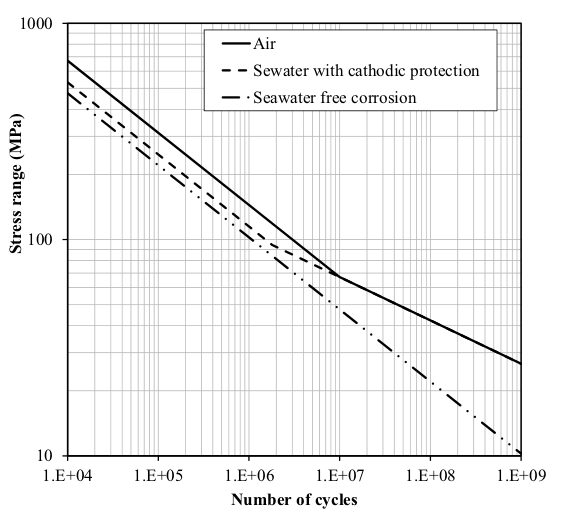
\includegraphics[width=0.5\linewidth]{figures/sn_tubular.png}
%    \caption{W\"ohler curves for tubular joints in different configurations (source: \cite{dnv_fatigue_2016})}
%    \label{fig:sn_curve}
%\end{figure}

Damage is a physical measure of the structure's fatigue. 
An approach to compute the damage, is to consider the fatigue contribution of each stress cycle according to the W\"ohler curve. 
Miner's rule defines a damage by summing the fatigue contributions of the stress cycles:
\begin{equation}
    y = \sum_{j=1}^{k} \frac{1}{N_{\mathrm{c}}^{(j)}} = \sum_{j=1}^{k} \frac{1}{W\left(s^{(j)}\right)}
    %d = \sum_{i=1}^{k} \frac{n_i}{N_{\mathrm{c}}_i} = \sum_{i=1}^{k} \frac{n_i}{W(s_i)}
    \label{miner}
\end{equation}

When using Miner's rule, an alternative is to use bins to classify the stress ranges as an histogram. 
Our intuition is that choosing a number of bins too small will lead to a poor approximation of the damage. 
\cite{dnv_fatigue_2016} standards recommend to use at least 20 bins for damage computation. 
Few tests were performed on a defined simulation model, for a fixed input stress time serie. 
A reference damage was computed by applying the Miner's rule to all stress range identified by rainflow counting ($\{n_i = 1\}_{i=1}^k$). 
Then, for various numbers of bins, stress ranges were classified and Miner's rule applied to these classes. 
The conclusion is that this method leads to a relative error around 1\% for 500 bins. 




%============================================================%
%============================================================%
\section{Design and operation practices} \label{sec:owt_design}
%============================================================%
%============================================================%


%============================================================%
\subsection{Preliminary design}
%============================================================%
    \begin{itemize}
        \item Different parts of the turbine (monopile, transition piece, fundation, tower), different turbine designs
        \item What are the key steps for a wind farm project in France 
        \item Pre-installation measures are usually done for a period of 1 to 3 year. This data is often validated against long-term regional datasets \cite{sempreviva_2008_wind_assessment_review}. Note that floating lidars present an opportunity \elias{add ref}
        \item general design from IEC61400 with part 1 and part 3
        \item Different designs : soft-stiff, stiff-stiff 
        \item Design load cases 
        \item How does it work : different ranges of function depending on the wind speed (cut-in, cut-off)
        \item 
    \end{itemize}

%============================================================%
\subsection{Further design considerations}
%============================================================%
Various aspects should be taken into consideration during the design and installation of an offshore wind farm.


\paragraph{Soil modeling}
%------------------------------------------------------------%

\paragraph{Marine growth}
%------------------------------------------------------------%

\paragraph{Global scour}
%------------------------------------------------------------%

\paragraph{Port logistics}
%------------------------------------------------------------%

\paragraph{Grid impact}
%------------------------------------------------------------%

\paragraph{Environmental impact and social acceptance} 
%------------------------------------------------------------%

\paragraph{Manufacturing quality inducing stress concentration factor}
%------------------------------------------------------------%



%============================================================%
\subsection{Maintenance and end-of-life management}
%============================================================%
\begin{itemize}
    \item Operation and maintenance
    \item Repowering vs. revamping
    \item Recycling 
\end{itemize}


%============================================================%
%============================================================%
\section{Uncertain inputs} \label{sec:owt_uncertainties}
%============================================================%
%============================================================%


\elias{Ref: Floating lidar as an advancedoffshore wind speed measurementtechnique: current technologystatus and gap analysis in regardto full maturity}
%============================================================%
\subsection{Environmental inputs}
%============================================================%

\elias{Add table}

\elias{The available data}

%============================================================%
\subsection{System inputs}
%============================================================%

\elias{Add table}

%============================================================%
\subsection{Probabilistic fatigue assessment}
%============================================================%




%============================================================%
%============================================================%
\section{Conclusion}
%============================================================%
%============================================================%